\section{程序功能介绍及实现思路}
该游戏以绘图库VS2019+EasyX\_20200902为基础,结合热门手游王者荣耀,制作而成的王者荣耀连连看。

编程以不同的界面为基础,分为4个模块,分别为菜单界面、游戏界面、游戏设置界面、排名界面。程序进入主函数后,通过全局参数的改变在函数Menu()、GamePlay()、setting()、RankInit()之间跳转,代码如下所示。

\lstset{language=C}
\begin{lstlisting}
int main() {
    initgraph(900, 580);
    begin:
    dataInit();
    Menu();
    if (menu_choose == 0) {
        GameInit();
        GamePlay();
        goto begin;
    }
    else if (menu_choose == 1) {
        setting();
        goto begin;
    }
    else if (menu_choose == 2) {
        RankInit();
        goto begin;
    }
    else if (menu_choose == 3) {
    }
    closegraph();
    return 0;
}
\end{lstlisting}

接下来一一介绍各个功能模块的设计和实现思路。

\subsection{菜单界面设计}
\subsubsection{功能介绍}
该界面是用户开启软件的后直接出现的菜单界面,如图\ref{fig:usemain}所示。

菜单界面有5个可用按键,分别用于进入游戏界面、游戏设置界面、排名界面和游戏充值,其中游戏充值是本游戏的特色功能,充值后英雄会换上皮肤,游戏中点击提示会有特别效果,基础得分加100。当鼠标放在对应可点击区域时,对应区域会出现高亮提示。这部分界面设计和代码实现参考EasyX参考项目数独\footnote{https://codebus.cn/chenh/a/sudoku}。

\begin{figure}[!htbp]
% \begin{figure}[H]
    \centering
    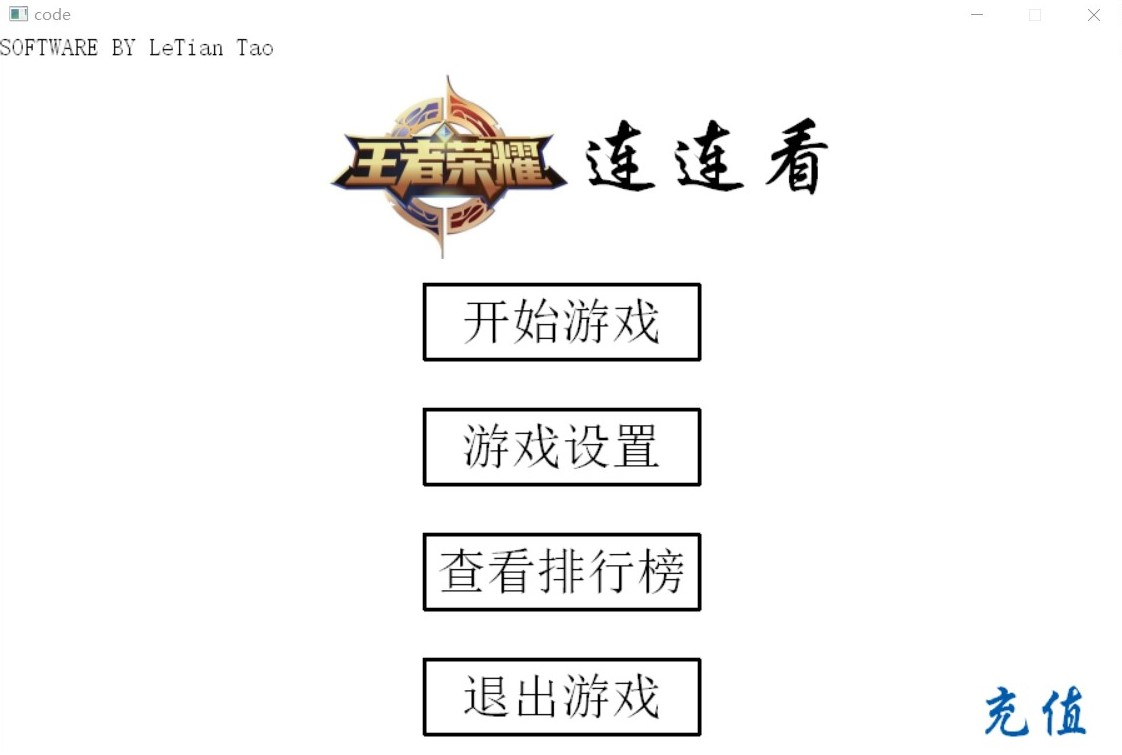
\includegraphics[width=0.6\textwidth]{usemain.jpg}
    \caption{菜单界面} \label{fig:usemain}
\end{figure}

\subsubsection{实现思路}
\paragraph{高亮显示}
在Menu()函数中运行一个死循环,每次循环通过msg.GetMouseMsg().x和msg.GetMouseMsg().y获取鼠标位置,msg是一个MOUSEMSG类型变量,MOUSEMSG用于给出鼠标信息,在<graphics.h>库中给出。获取鼠标位置信息后,每循环对相关显示参数(如字体颜色、边框颜色)进行刷新,从而鼠标在特定位置时,对应点击区域后出现高亮显示。
\paragraph{点击操作}

当msg.uMsg为WM\_LBUTTONUP,即鼠标为点击操作时,判断鼠标位置是否在对应区域,是则设置全局变量,跳出循环,通过设置的全局变量进入下一个界面。

\subsection{游戏界面设计}
\subsubsection{功能介绍}
该界面是玩家玩游戏的界面,如图\ref{fig:play}所示。游戏界面分为游戏区域和设置区域。

游戏区域会显示10*14的头像,在英雄池中有50个英雄,每次游戏会选择13个英雄,在主界面点击充值后,所以英雄会换上皮肤。

设置区域显示得分、提示次数、洗牌次数、剩余游戏时间。点击提示会消去一对图片,充值后能连环消去多个图片,点击洗牌会随机洗牌,点击退出回到主界面,当对应提示、洗牌次数为0时,程序也进行了保护。每次正确消除会得到两分加成,当玩家连续两次消除小于两秒时,得分处会显示DOUBLE,得分加倍,不同难度的关卡设置的加成分数也不一样。

\begin{figure}[!htbp]
% \begin{figure}[H]
    \centering
    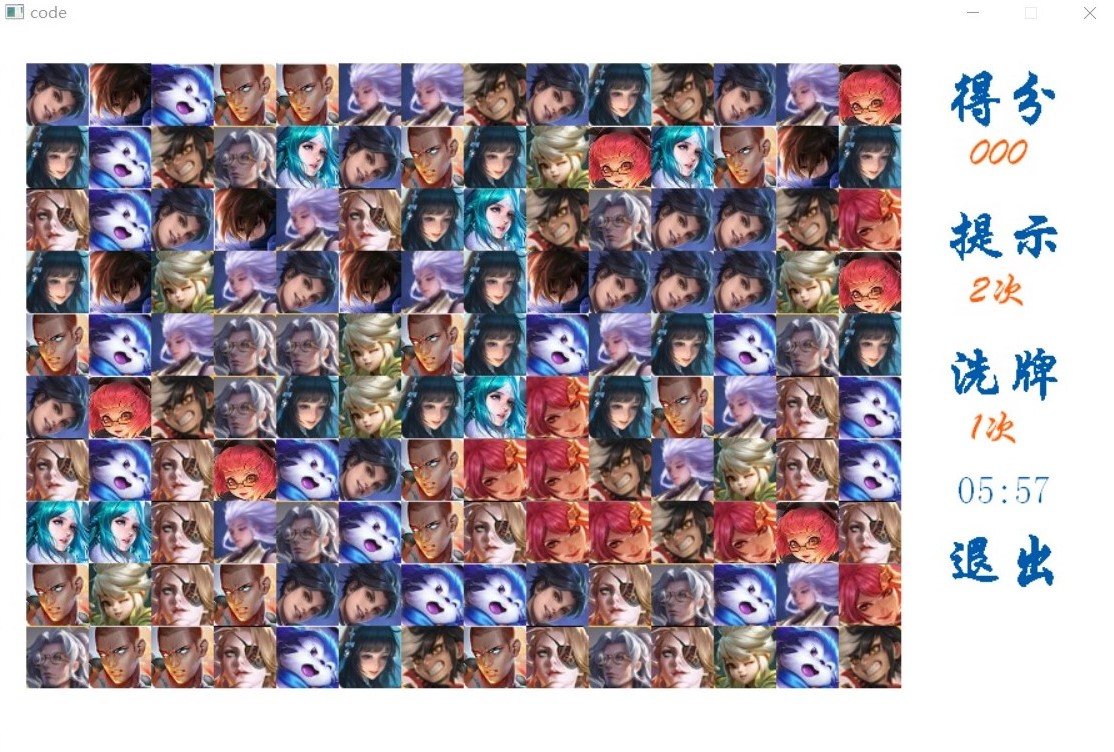
\includegraphics[width=0.6\textwidth]{play.jpg}
    \caption{游戏界面} \label{fig:play}
\end{figure}

\subsubsection{实现思路}
\paragraph{加载图片}
程序在ImportImage()用loadimage(\&img[0], L"./fig/0.jpg", box\_width, box\_width)加载图片,输入参数为待加载的图片变量指针,图片路径,图片大小。对充值用户,在另一个文件夹中获取带有皮肤的英雄图片。每次加载图片50张,但每次只选择13张作为每次游戏的图片。这通过1000次随机交换对应图片实现。交换图片代码如下,这里多次交换代替随机打乱的思路在程序中多次用到,例如点击洗牌后的效果和下述图片生成的方法。
\lstset{language=C}
\begin{lstlisting}
int i, j, T = 1000;
IMAGE tmp;
while (T--)
{
    i = rand() % 50+1;
    j = rand() % 50+1;

    tmp = img[i];
    img[i] = img[j];
    img[j] = tmp;
}
\end{lstlisting}

\paragraph{图片生成}
在GameInit()中生成图片,为了保障可解性,我在图像的上半区的每个位置随机选择一个英雄放入1维数组MAP。MAP用于储存各个位置的图片标签,可以通过MAP[x , max\_col * y]访问到各个位置的图片。下半区直接复制上半区,并并进行100次的随机交换作为随机打乱。有趣的是,当随机交换次数为1000次时,上下部分出现的图片大部分相同,没有达到打乱效果,交换100次打乱效果较好。因此,这里通过随机一般图片-直接复制-随机交换实现了可解性。打乱后对相邻图片进行判断,相邻相同图片小于10个则会重新生成。

\paragraph{可连性判断}
消除思路参考知乎:C++连连看教程\footnote{https://zhuanlan.zhihu.com/p/59069810}。总体思路是将三段连接判断is\_connect\_three()分解为其中一点位置十字区域内是否存在点和另一点二段连接,二段连接判断is\_connect\_two()分解为是否能通过矩形对角点和另一点一段连接,而图像的一段连接is\_connect\_one()分解为横向连接和纵向连接,即两点之间是否全部为空白进行判断。在判断两点连接性时,通过is\_connect一次调用三种可连性判断函数进行判决。

\paragraph{消去动画}
当成功连接两点时,对应路径上会出现一条系统判断的消去路径。此路径的绘制和消去耗费了我很多精力。简单的思路就是在显示路径后,将需要消去的点存入全局变量clear\_list,等待200ms后消去,同时这200ms也是加倍得分DOUBLE显示的时间。由于在可连续判断时,多层函数调用,因此很难理清这些线是否需要连接,点是否真需要删除,因此在is\_connect()传入两个点坐标的同时,也传输参数is\_draw判断是否需要绘制点。这里的消去动画设置逻辑复杂,且没有移植性,因此不做详细介绍。从代码优化的角度看,我觉得这里的代码虽然实现了消去效果,但是不够优雅,值得进一步优化。

\paragraph{提示功能}
点击提示时,程序会从左上角开始,每个点一次判断和其后的点的可连接性。一开始我找到第一个点没有及时break导致较多点对被消除,因此我把这个BUG修改成充值后的提示效果。这里的二重遍历也在每一次消除后判断图中是否还有可连接的点,不能继续连接就会进行自动洗牌。但程序从未跑到出现不可连接的情况,因此这部分程序一直没有得到测试。

\subsection{游戏设置界面设计}
\subsubsection{功能介绍}
通过改变英雄数量提高游戏难度,基础数量为13,可以选择13、15、17个英雄,三者在快速消去时分别可获得4、5、6分的加成。
% 设置界面如图\ref{fig:setting}所示。

% \begin{figure}[!htbp]
%     \centering
%     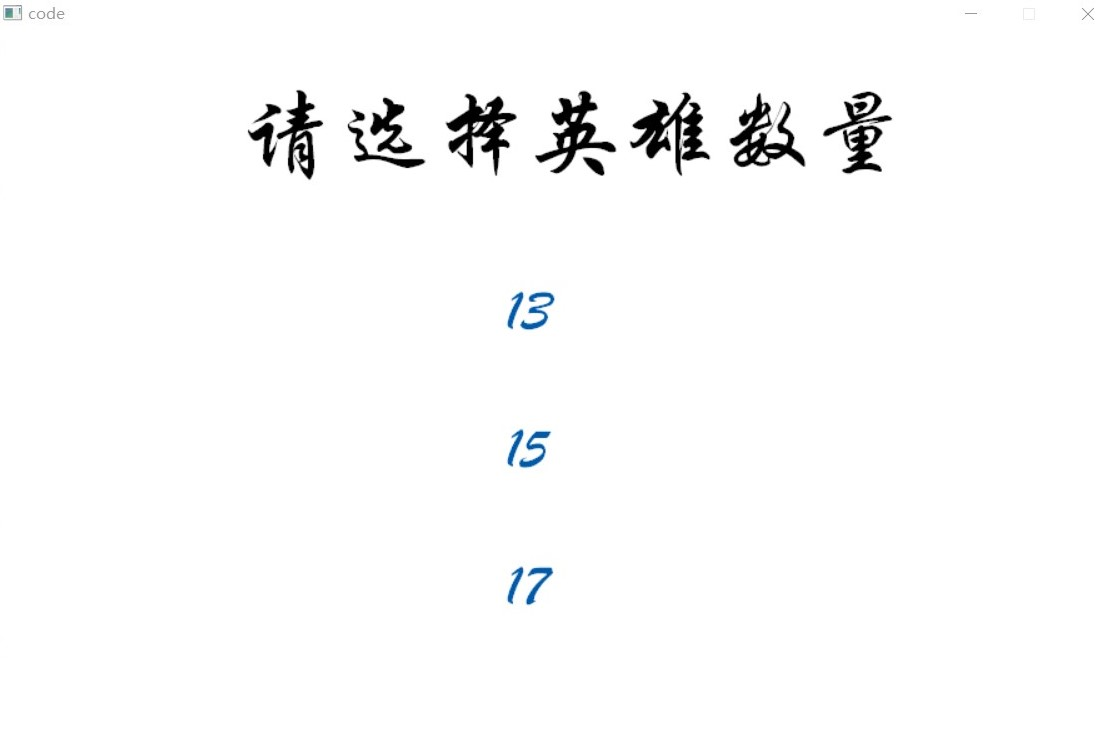
\includegraphics[width=0.6\textwidth]{setting.jpg}
%     \caption{游戏界面} \label{fig:setting}
% \end{figure}

\subsubsection{实现思路}
通过改变全局变量num\_hero改变英雄数量。

\subsection{排名界面设计}
\subsubsection{功能介绍}
读取记录分数的txt文件,显示排行榜。
% 界面如图\ref{fig:rank}所示。
% \begin{figure}[!htbp]
%     \centering
%     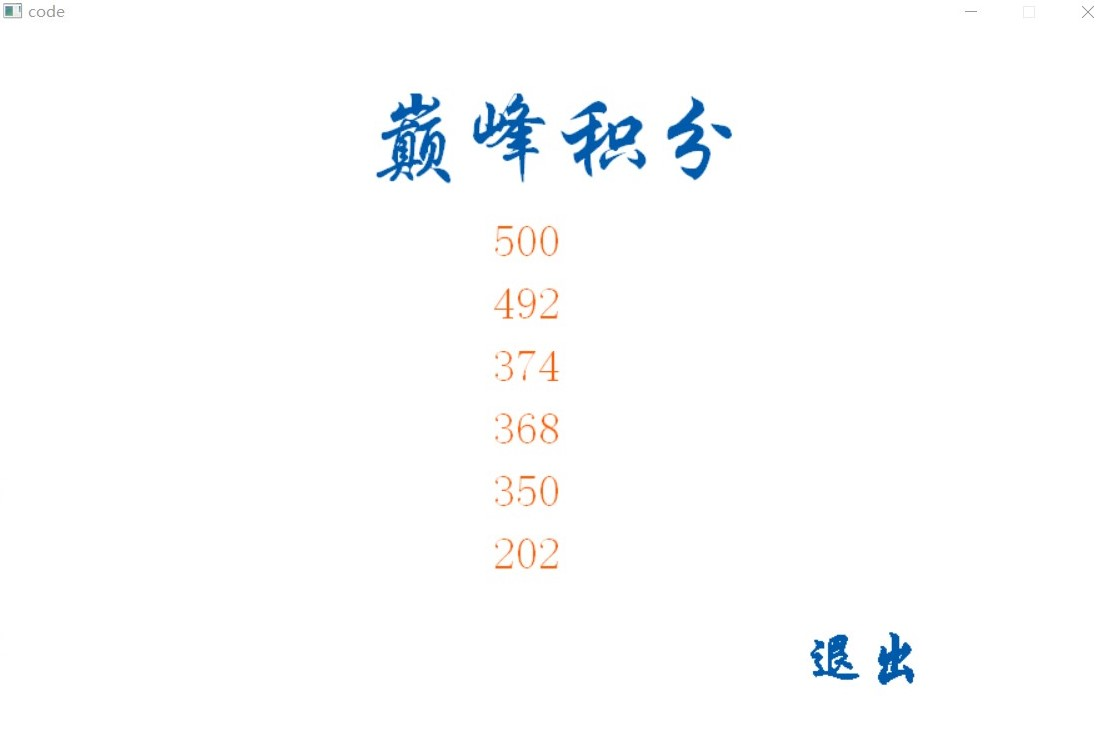
\includegraphics[width=0.6\textwidth]{rank.jpg}
%     \caption{游戏界面} \label{fig:rank}
% \end{figure}

\subsubsection{实现思路}
这里采用fscanf\_s进行文件读取,再通过冒泡排序一次排行,最终只显示前8名。文件读取和排序代码如下:
\lstset{language=C}
\begin{lstlisting}
err = fopen_s(&stream, "score.txt", "a+");
char ch = 'c';
int term = 0;
while (ch != EOF) {
    fscanf_s(stream, "%d", &time_rank[term]);
    ch = fgetc(stream);
    term++;
}
int temp;
for (int i = 0; i < term-2 ; i++) {
    int isSorted = 1; 
    for (int j = 0; j < term-2 -i; j++) {
        if (time_rank[j] < time_rank[j + 1]) {
            temp = time_rank[j];
            time_rank[j] = time_rank[j + 1];
            time_rank[j + 1] = temp;
            isSorted = 0; 
            }
        }
        if (isSorted) break;
}
\end{lstlisting}

类似地,每次胜利后将分数写入文件的代码如下:
\lstset{language=C}
\begin{lstlisting}
FILE* stream;
errno_t err;
err = fopen_s(&stream, "score.txt", "a+");
fprintf(stream, "%d\n", score);
_fcloseall();
\end{lstlisting}




